\documentclass[border=4pt,12pt]{standalone}
% House style for redrawn exam diagrams (diagram-v4: 0.4pt lines, filled -latex arrows, fine dashes; stipple and hatching drawn as real dots/lines (no PDF/SVG patterns, so they render in every browser and at any scale); transparent background). Every figure \input's this.
\usepackage{amsmath,amssymb}
\usepackage{txfonts}
\usepackage{pdfrender,xcolor}
% \halo{text}: label on shading. The shading stops just around each letter's outline (a thin knock-out that follows the
% glyphs, like the papers' typesetting), never a box. Owner: "I don't want a box around the text".
\newcommand{\halo}[1]{\leavevmode\rlap{\pdfrender{TextRenderingMode=2,LineWidth=2.2pt,LineJoinStyle=1,StrokeColor=white,FillColor=white}#1}#1}
\usepackage{tikz,pgfplots}
\pgfplotsset{compat=1.18}
\usetikzlibrary{arrows.meta,calc,angles,quotes,patterns,patterns.meta,intersections,positioning,decorations.markings,shapes.geometric}
% Stipple and hatching are drawn as actual dots / lines clipped to the region (path picture), NOT as pattern fills:
% SVG <pattern> fills vanish or blur when browsers scale the image, so the owner could not see the shading.
% Each dot is a 0.72pt square (keeps SVGs small; reads as a dot at print size). Dots sit on one global staggered grid, so neighbouring regions line up.
\makeatletter
\newdimen\ex@x \newdimen\ex@y \newdimen\ex@xa \newdimen\ex@ya \newdimen\ex@xb \newdimen\ex@yb \newcount\ex@row
\def\exam@stipplecolor{black!75}\def\exam@dotr{0.42pt}\def\exam@dotgap{2.5}
\def\ex@rowdots{\ifdim\ex@x<\ex@xb \pgfpathrectangle{\pgfqpoint{\dimexpr\ex@x-0.36pt\relax}{\dimexpr\ex@y-0.36pt\relax}}{\pgfqpoint{0.72pt}{0.72pt}}\advance\ex@x by \exam@dotgap pt\relax\expandafter\ex@rowdots\fi}
\def\exam@stipple{%
  \pgftransformreset% dots are sized in real points even inside scaled pictures
  \pgfpointanchor{path picture bounding box}{south west}\ex@xa=\pgf@x \ex@ya=\pgf@y
  \pgfpointanchor{path picture bounding box}{north east}\ex@xb=\pgf@x \ex@yb=\pgf@y
  \pgfsetfillcolor{\exam@stipplecolor}\pgfmathsetmacro\ex@h{\exam@dotgap/2}%
  \pgfmathtruncatemacro\ex@r{floor(\ex@ya/\ex@h)-1}\ex@row=\ex@r\relax
  \ex@y=\ex@r\dimexpr\ex@h pt\relax
  \loop\ifdim\ex@y<\ex@yb
    \pgfmathtruncatemacro\ex@c{floor(\ex@xa/\exam@dotgap)-1}\ex@x=\ex@c\dimexpr\exam@dotgap pt\relax
    \ifodd\ex@row \advance\ex@x by \ex@h pt\fi
    \ex@rowdots
    \advance\ex@y by \ex@h pt \advance\ex@row by 1
    \ifnum\numexpr\ex@row-(\ex@row/4)*4\relax=0 \pgfusepath{fill}\fi% flush every 4 rows: bounded TeX memory, few clip copies in the SVG
  \repeat\pgfusepath{fill}}
\newdimen\ex@d
\def\exam@hatch#1{% #1 = 1 for /, -1 for \ ; lines 45 degrees, 3pt apart
  \pgftransformreset
  \pgfpointanchor{path picture bounding box}{south west}\ex@xa=\pgf@x \ex@ya=\pgf@y
  \pgfpointanchor{path picture bounding box}{north east}\ex@xb=\pgf@x \ex@yb=\pgf@y
  \ex@d=\dimexpr\ex@yb-\ex@ya\relax \ex@x=\dimexpr\ex@xa-\ex@d\relax
  \loop\ifdim\ex@x<\ex@xb
    \ifnum#1>0 \pgfpathmoveto{\pgfqpoint{\ex@x}{\ex@ya}}\pgfpathlineto{\pgfqpoint{\dimexpr\ex@x+\ex@d\relax}{\ex@yb}}%
    \else \pgfpathmoveto{\pgfqpoint{\ex@x}{\ex@yb}}\pgfpathlineto{\pgfqpoint{\dimexpr\ex@x+\ex@d\relax}{\ex@ya}}\fi
    \advance\ex@x by 4.24pt
  \repeat
  \pgfsetlinewidth{0.4pt}\pgfsetstrokecolor{black}\pgfusepath{stroke}}
\def\examstipple{\exam@stipple}\def\examhatch{\exam@hatch}\def\examsetstipplecolor#1{\def\exam@stipplecolor{#1}}\def\examsetdotgap#1{\def\exam@dotgap{#1}}
\makeatother
% (legacy pattern kept for old files)
% staggered stipple like the NESA papers' dotted shading
\pgfdeclarepatternformonly{exam stipple}{\pgfpointorigin}{\pgfqpoint{2.2pt}{2.2pt}}{\pgfqpoint{2.2pt}{2.2pt}}{%
  \pgfpathcircle{\pgfqpoint{0.55pt}{0.55pt}}{0.42pt}\pgfpathcircle{\pgfqpoint{1.65pt}{1.65pt}}{0.42pt}\pgfusepath{fill}}
\tikzset{
  every picture/.style={line width=0.6pt, >={Latex[length=2mm,width=1.3mm]}},
  curve/.style={line width=0.6pt},
  open arrow/.style={-{Latex[length=2mm,width=1.3mm]}},  % owner: filled -latex heads everywhere, no open chevrons
  aux/.style={dash pattern=on 2pt off 1.5pt, line width=0.6pt},
  shade/.code={\def\exA{#1}\def\exB{none}\ifx\exA\exB\else\pgfkeysalso{fill=black!18}\fi},
  shade/.default=on,
  shade dots/.style={fill=none, path picture={\examstipple}},
  stipple color/.code={\examsetstipplecolor{#1}},
  stipple gap/.code={\examsetdotgap{#1}},
  shade dense dots/.style={fill=none, stipple gap=1.6, path picture={\examstipple}},
  shade hatch/.style={fill=none, path picture={\examhatch{1}}},
  shade hatch reverse/.style={fill=none, path picture={\examhatch{-1}}},
  shade solid/.style={fill=black},
  pt/.style={circle, fill, inner sep=1.1pt},
  open pt/.style={circle, draw, fill=white, inner sep=1.1pt},
}
\pgfplotsset{
  exam axes/.style={axis lines=middle, axis line style={->}, xlabel={$x$}, ylabel={$y$},
    xlabel style={anchor=west}, ylabel style={anchor=south}, tick label style={font=\small},
    every axis plot/.append style={line width=0.6pt, black}, samples=200, clip=false,
    enlargelimits=false, axis on top},
}

\begin{document}
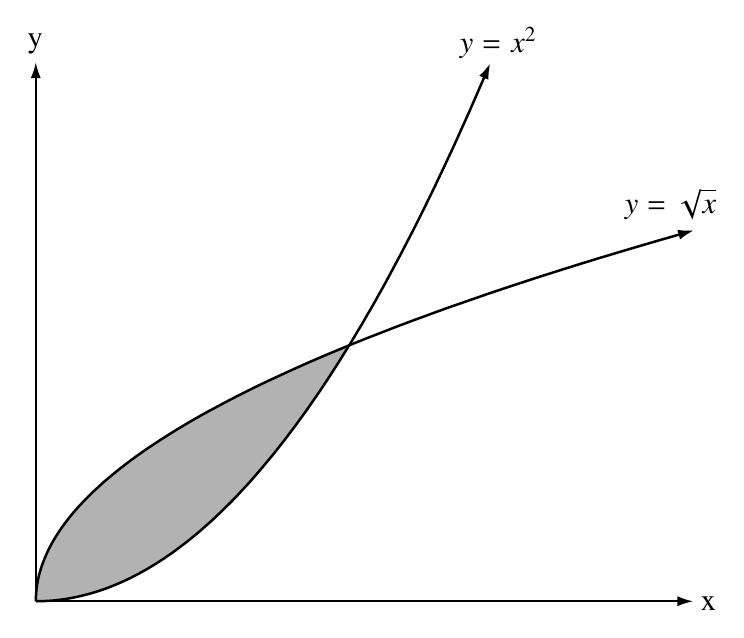
\begin{tikzpicture}[x=0.0127cm,y=-0.0127cm,font=\fontsize{11}{13}\selectfont]
\fill[black!30] plot[smooth] coordinates {(56.5,605.0) (56.6,600.7) (56.9,596.3) (57.3,592.0) (57.9,587.6) (58.8,583.3) (59.7,579.0) (60.9,574.6) (62.3,570.3) (63.8,565.9) (65.5,561.6) (67.4,557.3) (69.5,552.9) (71.7,548.6) (74.2,544.3) (76.8,539.9) (79.6,535.6) (82.5,531.2) (85.7,526.9) (89.0,522.6) (92.5,518.2) (96.2,513.9) (100.1,509.5) (104.1,505.2) (108.4,500.9) (112.8,496.5) (117.4,492.2) (122.2,487.8) (127.1,483.5) (132.2,479.2) (137.6,474.8) (143.0,470.5) (148.7,466.2) (154.6,461.8) (160.6,457.5) (166.8,453.1) (173.2,448.8) (179.8,444.5) (186.5,440.1) (193.5,435.8) (200.6,431.4) (207.9,427.1) (215.4,422.8) (223.0,418.4) (230.9,414.1) (238.9,409.7) (247.1,405.4) (255.4,401.1) (264.0,396.7) (272.7,392.4) (281.7,388.1) (290.7,383.7) (300.0,379.4) (309.5,375.0) (319.1,370.7) (328.9,366.4) (338.9,362.0) (349.1,357.7) (359.5,353.3) (370.0,349.0) (370.0,349.0) (364.7,357.6) (359.4,366.1) (354.1,374.4) (348.7,382.5) (343.4,390.6) (338.1,398.4) (332.8,406.1) (327.5,413.7) (322.2,421.1) (316.9,428.4) (311.6,435.6) (306.2,442.5) (300.9,449.4) (295.6,456.1) (290.3,462.6) (285.0,469.0) (279.7,475.3) (274.4,481.4) (269.0,487.3) (263.7,493.1) (258.4,498.8) (253.1,504.3) (247.8,509.7) (242.5,514.9) (237.2,520.0) (231.8,524.9) (226.5,529.7) (221.2,534.3) (215.9,538.8) (210.6,543.2) (205.3,547.3) (200.0,551.4) (194.7,555.3) (189.3,559.0) (184.0,562.6) (178.7,566.1) (173.4,569.4) (168.1,572.6) (162.8,575.6) (157.5,578.5) (152.1,581.2) (146.8,583.7) (141.5,586.2) (136.2,588.5) (130.9,590.6) (125.6,592.6) (120.3,594.4) (114.9,596.1) (109.6,597.6) (104.3,599.0) (99.0,600.3) (93.7,601.4) (88.4,602.4) (83.1,603.2) (77.8,603.8) (72.4,604.3) (67.1,604.7) (61.8,604.9) (56.5,605.0)} -- cycle;
\draw[->] (56.5,605) -- (714,605);
\draw[->] (56.5,605) -- (56.5,66);
\node[anchor=base,inner sep=0] at (729.5,614) {x};
\node[anchor=base,inner sep=0] at (56,51.5) {y};
\draw[->, line width=0.9pt] plot[smooth] coordinates {(56.5,605.0) (64.8,604.8) (73.1,604.3) (81.3,603.4) (89.5,602.2) (97.6,600.6) (105.7,598.7) (113.7,596.5) (121.6,594.0) (129.4,591.2) (137.1,588.1) (144.7,584.8) (152.1,581.2) (159.5,577.4) (166.7,573.4) (173.9,569.1) (180.9,564.7) (187.8,560.1) (194.6,555.4) (201.2,550.4) (207.8,545.4) (214.2,540.2) (220.6,534.9) (226.8,529.4) (233.0,523.9) (239.0,518.2) (245.0,512.4) (250.9,506.6) (256.7,500.7) (262.3,494.6) (268.0,488.5) (273.5,482.4) (278.9,476.1) (284.3,469.8) (289.6,463.4) (294.9,457.0) (300.0,450.5) (305.1,444.0) (310.1,437.4) (315.1,430.8) (320.0,424.1) (324.9,417.4) (329.7,410.6) (334.4,403.8) (339.1,397.0) (343.7,390.1) (348.3,383.2) (352.8,376.3) (357.3,369.3) (361.7,362.3) (366.1,355.3) (370.5,348.2) (374.8,341.1) (379.0,334.0) (383.3,326.9) (387.4,319.7) (391.6,312.6) (395.7,305.4) (399.7,298.1) (403.8,290.9) (407.8,283.6) (411.7,276.3) (415.6,269.0) (419.5,261.7) (423.4,254.4) (427.2,247.0) (431.0,239.7) (434.8,232.3) (438.5,224.9) (442.2,217.5) (445.9,210.1) (449.5,202.6) (453.2,195.2) (456.8,187.7) (460.3,180.2) (463.9,172.7) (467.4,165.2) (470.9,157.7) (474.4,150.2) (477.8,142.7) (481.2,135.1) (484.6,127.6) (488.0,120.0) (491.4,112.4) (494.7,104.8) (498.0,97.2) (501.3,89.6) (504.6,82.0) (507.8,74.4) (511.1,66.8)};
\draw[->, line width=0.9pt] plot[smooth] coordinates {(56.5,605.0) (56.9,596.2) (58.0,587.4) (59.8,578.7) (62.3,570.2) (65.4,562.0) (69.0,553.9) (73.1,546.1) (77.7,538.5) (82.6,531.1) (87.9,524.0) (93.4,517.1) (99.2,510.5) (105.3,504.0) (111.5,497.7) (118.0,491.7) (124.5,485.7) (131.3,480.0) (138.1,474.4) (145.1,468.9) (152.1,463.6) (159.3,458.4) (166.5,453.3) (173.9,448.4) (181.3,443.5) (188.7,438.8) (196.2,434.1) (203.8,429.5) (211.4,425.0) (219.1,420.6) (226.8,416.3) (234.6,412.1) (242.4,407.9) (250.2,403.8) (258.1,399.7) (266.0,395.7) (273.9,391.8) (281.9,387.9) (289.9,384.1) (297.9,380.4) (305.9,376.7) (314.0,373.0) (322.0,369.4) (330.1,365.8) (338.2,362.3) (346.4,358.8) (354.5,355.4) (362.7,352.0) (370.9,348.6) (379.1,345.3) (387.3,342.0) (395.5,338.8) (403.8,335.6) (412.0,332.4) (420.3,329.2) (428.6,326.1) (436.9,323.0) (445.2,320.0) (453.5,316.9) (461.8,313.9) (470.1,310.9) (478.5,308.0) (486.8,305.1) (495.2,302.2) (503.5,299.3) (511.9,296.4) (520.3,293.6) (528.7,290.8) (537.1,288.0) (545.5,285.3) (553.9,282.5) (562.3,279.8) (570.8,277.1) (579.2,274.4) (587.6,271.8) (596.1,269.1) (604.5,266.5) (613.0,263.9) (621.4,261.3) (629.9,258.8) (638.4,256.2) (646.9,253.7) (655.3,251.2) (663.8,248.7) (672.3,246.2) (680.8,243.7) (689.3,241.3) (697.8,238.8) (706.3,236.4) (714.9,234.0)};
\node[anchor=base west,inner sep=0] at (480,56.5) {$y=x^{2}$};
\node[anchor=base west,inner sep=0] at (645,217) {$y=\sqrt{x}$};
\end{tikzpicture}
\end{document}
